\documentclass{article}
\usepackage{v-test-paper}
\begin{document}
\begin{enumerate}
    \item One end of a horizontal uniform beam of weight $W$ and length $L$ is hinged on a vertical wall at point $O$ and its other end is supported by a light inextensible rope. The other end of the rope is fixed at point $Q$, at a height $L$ above the hinge at point $O$. A block of weight $\alpha W$ is attached at the point $P$ of the beam, as shown in the figure (not to scale). The rope can sustain a maximum tension of $(2\sqrt{2})W$. Which of the following statement(s) is(are) correct?
    \begin{center}
        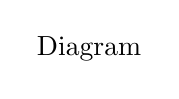
\begin{tikzpicture}
            \node {Diagram};
        \end{tikzpicture}
    \end{center}
        \begin{tasks}(1)
            \task The vertical component of reaction force at $O$ does not depend on $\alpha$
            \task The horizontal component of reaction force at $O$ is equal to $W$ for $\alpha = 0.5$
            \task The tension in the rope is $2W$ for $\alpha = 0.5$
            \task The rope breaks if $\alpha > 1.5$
        \end{tasks}
        
    \item A source, approaching with speed $u$ towards the open end of a stationary pipe of length $L$, is emitting a sound of frequency $f_s$. The farther end of the pipe is closed. The speed of sound in air is $v$ and $f_0$ is the fundamental frequency of the pipe. For which of the following combination(s) of $u$ and $f_s$, will the sound reaching the pipe lead to a resonance?
        \begin{tasks}(2)
            \task $ u = 0.8v $ and $ f_s = f_0 $
            \task $ u = 0.8v $ and $ f_s = 2f_0 $
            \task $ u = 0.8v $ and $ f_s = 0.5f_0 $
            \task $ u = 0.5v $ and $ f_s = 1.5f_0 $
        \end{tasks}

    \item For a prism of prism angle $\theta = 60^{\circ}$, the refractive indices of the left half and the right half are, respectively, $n_1$ and $n_2$ ($n_2 \geq n_1$) as shown in the figure. The angle of incidence $i$ is chosen such that the incident light rays will have minimum deviation if $n_1 = n_2 = n = 1.5$. For the case of unequal refractive indices, $n_1 = n$ and $n_2 = n + \Delta n$ (where $\Delta n \ll n$), the angle of emergence $e = i + \Delta e$. Which of the following statement(s) is(are) correct?
        \begin{center}
            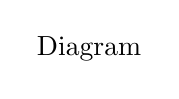
\begin{tikzpicture}
                \node {Diagram};
            \end{tikzpicture}
        \end{center}
        \begin{tasks}(1)
            \task The value of $\Delta e$ (in radians) is greater than that of $\Delta n$.
            \task $\Delta e$ is proportional to $\Delta n$.
            \task $\Delta e$ lies between 2.0 and 3.0 milliradians, if $\Delta n = 2.8 \times 10^{-3}$.
            \task $\Delta e$ lies between 1.0 and 1.6 milliradians, if $\Delta n = 2.8 \times 10^{-3}$.
        \end{tasks}
    \item A physical quantity $\vec{S}$ is defined as $\vec{S} = (\vec{E} \times \vec{B})/\mu_0$, where $\vec{E}$ is electric field, $\vec{B}$ is magnetic field and $\mu_0$ is the permeability of free space. The dimensions of $\vec{S}$ are the same as the dimensions of which of the following quantity(ies)?
        \begin{tasks}(2)
            \task $\dfrac{\text{Energy}}{\text{Charge} \times \text{Current}}$
            \task $\dfrac{\text{Force}}{\text{Length} \times \text{Time}}$
            \task $\dfrac{\text{Energy}}{\text{Volume}}$
            \task $\dfrac{\text{Power}}{\text{Area}}$
        \end{tasks}
    \item A heavy nucleus $N$, at rest, undergoes fission $N \rightarrow P + Q$, where $P$ and $Q$ are two lighter nuclei. Let $\delta M = M_N - M_P - M_Q$, where $M_P$, $M_Q$ and $M_N$ are the masses of $P$, $Q$ and $N$, respectively. $E_P$ and $E_Q$ are the kinetic energies of $P$ and $Q$, respectively. The speeds of $P$ and $Q$ are $v_P$ and $v_Q$, respectively. If $c$ is the speed of light, which of the following statement(s) is(are) correct?
    \begin{tasks}(1)
        \task $E_P + E_Q = c^2 \delta$
        \task $E_P = \left( \frac{M_P}{M_P+M_Q} \right) c^2 \delta$
        \task $\frac{v_P}{v_Q} = \frac{M_Q}{M_P}$
        \task The magnitude of momentum for $P$ as well as $Q$ is $c \sqrt{2\mu \delta}$, where $\mu = \frac{M_P M_Q}{M_P+M_Q}$
    \end{tasks}

    \item Two concentric circular loops, one of radius $R$ and the other of radius $2R$, lie in the xy-plane with the origin as their common center, as shown in the figure. The smaller loop carries current $I_1$ in the anti-clockwise direction and the larger loop carries current $I_2$ in the clockwise direction, with $I_2 > 2I_1$. $B(x,y)$ denotes the magnetic field at a point $(x,y)$ in the xy-plane. Which of the following statement(s) is(are) correct?
    \begin{center}
        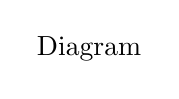
\begin{tikzpicture}
            \node {Diagram};
        \end{tikzpicture}
    \end{center}
        \begin{tasks}(1)
            \task $ B(x,y) $ is perpendicular to the xy-plane at any point in the plane
            \task $ |B(x,y)| $ depends on $ x $ and $ y $ only through the radial distance $ r = \sqrt{x^2 + y^2} $
            \task $ |B(x,y)| $ is non-zero at all points for $ r < R $
            \task $ \vec{B}(x,y) $ points normally outward from the xy-plane for all the points between the two loops
        \end{tasks}



\textbf{Question Stem}

    A soft plastic bottle, filled with water of density 1 \text{gm/cc}, carries an inverted glass test-tube with some air (ideal gas) trapped as shown in the figure. The test-tube has a mass of 5 \text{gm}, and it is made of a thick glass of density 2.5 \text{gm/cc}. Initially the bottle is sealed at atmospheric pressure $p_0 = 10^5$ \text{Pa} so that the volume of the trapped air is $v_0 = 3.3$ \text{cc}. When the bottle is squeezed from outside at constant temperature, the pressure inside rises and the volume of the trapped air reduces. It is found that the test tube begins to sink at pressure $p_0 + \Delta p$ without changing its orientation. At this pressure, the volume of the trapped air is $v_0 - \Delta v$. Let $\Delta v = X$ \text{cc} and $\Delta p = Y \times 10^3$ \text{Pa}.
    \begin{center}
        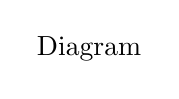
\begin{tikzpicture}
            \node {Diagram};
        \end{tikzpicture}
    \end{center}
    \item The value of $X$ is $\hrulefill$ .
    \item The value of $Y$ is $\hrulefill$ .


\textbf{Question Stem}

    A pendulum consists of a bob of mass $m = 0.1 \, \text{kg}$ and a massless inextensible string of length $L = 1.0 \, \text{m}$. It is suspended from a fixed point at height $H = 0.9 \, \text{m}$ above a frictionless horizontal floor. Initially, the bob of the pendulum is lying on the floor at rest vertically below the point of suspension. A horizontal impulse $ P = 0.2 \, \text{kg}\cdot\text{m/s}$ is imparted to the bob at some instant. After the bob slides for some distance, the string becomes taut and the bob lifts off the floor. The magnitude of the angular momentum of the pendulum about the point of suspension just before the bob lifts off is $j \, \text{kg}\cdot\text{m}^2/\text{s}$. The kinetic energy of the pendulum just after the lift-off is $K \, \text{Joules}$.

    \item The value of $j$ is \_\_\_.
    \item The value of $K$ is \_\_\_.


\textbf{Question Stem}

    In a circuit, a metal filament lamp is connected in series with a capacitor of capacitance $C \, \mu F$ across a $200 \, V$, $50 \, Hz$ supply. The power consumed by the lamp is $500 \, W$ while the voltage drop across it is $100 \, V$. Assume that there is no inductive load in the circuit. Take $ \text{rms} $ values of the voltages. The magnitude of the phase-angle (in degrees) between the current and the supply voltage is $\phi$. Assume, $\pi\sqrt{3} \approx 5$.


    \item The value of $C$ is \_\_\_.
    \item The value of $\phi$ is \_\_\_.


\begin{center}
    \textsc{Comprehension Based Questions}
\end{center}

    A special metal S conducts electricity without any resistance. A closed wire loop, made of S, does not allow any change in flux through itself by inducing a suitable current to generate a compensating flux. The induced current in the loop cannot decay due to its zero resistance. This current gives rise to a magnetic moment which in turn repels the source of magnetic field or flux. Consider such a loop, of radius a, with its center at the origin. A magnetic dipole of moment $\vec{m}$ is brought along the axis of this loop from infinity to a point at distance $r>a$ from the center of the loop with its north pole always facing the loop, as shown in the figure below.
    
    The magnitude of magnetic field of a dipole $m$, at a point on its axis at distance $r$ is $$\frac{\mu_0}{4\pi}\frac{2m}{r^3},$$ where $\mu_0$ is the permeability of free space. The magnitude of the force between two magnetic dipoles with moments, $m_1$ and $m_2$, separated by a distance $r$ on the common axis, with their north poles facing each other, is $$\frac{k m_1 m_2}{r^4},$$ where $k$ is a constant of appropriate dimensions. The direction of this force is along the line joining the two dipoles.
    \begin{center}
        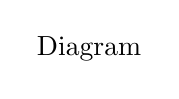
\begin{tikzpicture}
            \node {Diagram};
        \end{tikzpicture}
    \end{center}

    \item  When the dipole $m$ is placed at a distance $r$ from the center of the loop (as shown in the figure), the current induced in the loop will be 
    proportional to 
    \begin{tasks}(2)
        \task $m^3/r^3$ 
        \task $m^2/r^2$ 
        \task $m/r^2$ 
        \task $m/r$
    \end{tasks}
    \item The work done in bringing the dipole from infinity to a distance $r$ from the center of the loop by the given process is proportional to 
    \begin{tasks}(2)
        \task $m/r^5$ 
        \task $m^2/r^5$ 
        \task $m^2/r^7$ 
        \task $m/r^7$
    \end{tasks}



\begin{center}
    \textsc{Comprehension Based Questions}
\end{center}
    A thermally insulated cylinder has a thermally insulated and frictionless movable partition in the middle, as shown in the figure below. On each side of the partition, there is one mole of an ideal gas, with specific heat at constant volume, $C_v=2R$. Here, $R$ is the gas constant. Initially, each side has a volume $V_0$ and temperature $T_0$. The left side has an electric heater, which is turned on at very low power to transfer heat $Q$ to the gas on the left side. As a result, the partition moves slowly towards the right reducing the right side volume to $V_2$. Consequently, the gas temperatures on the left and the right sides become $T_1$ and $T_2$, respectively. Ignore the changes in the temperatures of the cylinder, heater and the partition.
    \begin{center}
        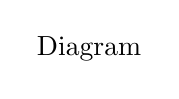
\begin{tikzpicture}
            \node {Diagram};
        \end{tikzpicture}
    \end{center}
    \item The value of $\frac{T_R}{T_0}$ is 
    \begin{tasks}(2)
        \task $\sqrt{2}$
        \task $\sqrt{3}$
        \task $2$
        \task $3$
    \end{tasks}


    \item The value of \(\frac{Q}{RT_0}\) is 
    \begin{tasks}(2)
        \task $4(2\sqrt{2}-1)$
        \task $4(2\sqrt{2}+1)$
        \task $5(2\sqrt{2}+1)$
        \task $5(2\sqrt{2}-1)$
    \end{tasks}



    \item In order to measure the internal resistance $ r_1 $ of a cell of emf $ E $, a meter bridge of wire resistance $ R_0 = 50 \, \Omega $, a resistance $ R_0/2 $, another cell of emf $ E/2 $ (internal resistance $ r $) and a galvanometer $ G $ are used in a circuit, as shown in the figure. If the null point is found at $ l = 72 \, \text{cm} $, then the value of $ r_1 $ is \_\_\_ $ \Omega $.
    
    \begin{center}
        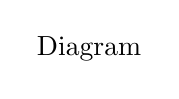
\begin{tikzpicture}
            \node {Diagram};
        \end{tikzpicture}
    \end{center}
    
    \item The distance between two stars of masses $ 3M $ and $ 6M $ is $ 9R $. Here $ R $ is the mean distance between the centers of the Earth and the Sun, and $ M_S $ is the mass of the Sun. The two stars orbit around their common center of mass in circular orbits with period $ nT $, where $ T $ is the period of Earth's revolution around the Sun. The value of $ n $ is \_\_\_.
    
    \item In a photoemission experiment, the maximum kinetic energies of photoelectrons from metals $P$, $Q$ and $R$ are $E_P$, $E_Q$ and $E_R$, respectively, and they are related by $E_P = 2E_Q = 2E_R$. In this experiment, the same source of monochromatic light is used for metals $P$ and $Q$ while a different source of monochromatic light is used for the metal $R$. The work functions for metals $P$, $Q$ and $R$ are $4.0 \, \text{eV}$, $4.5 \, \text{eV}$ and $5.5 \, \text{eV}$, respectively. The energy of the incident photon used for metal $R$, in $\text{eV}$, is \_\_\_.
    
\end{enumerate}
\end{document}